
\documentclass{report}
\usepackage[utf8]{inputenc}
\usepackage{graphicx}
\usepackage{subfigure}
\usepackage{subcaption}
\usepackage{biblatex}
\addbibresource{Citation.bib}
\usepackage{tabularx}
\usepackage{xcolor}
\usepackage[left= 1.8cm, right= 1.8cm, top=2cm, bottom=1.5cm]{geometry}
\usepackage{hyperref}

\begin{document}

\begin{center}
    
\includegraphics[width=10cm]{Logo-PNG.png}
\end{center}
\vspace{0.4cm}
\begin{center}
    \LARGE \textbf{Green University of Bangladesh} \\
    \large \textbf{Department of Computer Science and Engineering} \\
    \textbf{Faculty of Sciences and Engineering}\\
    \textbf{Semester: (Fall, Year:2022), B.Sc. in CSE(Day)}\\
    \vspace{1.5cm}
   \large \textbf{Project Report}\\
    \large \textbf{Course Title: Computer Networking Lab}\\
    \large \textbf{Course Code: CSE-312}\\
    \large \textbf{Section: PC 201 DB}\\
 \vspace{.8cm}
    \textbf{Project name:} Smart Irrigation System 
\vspace{1cm}

    \textbf{\underline{Student Details}}\\ 
     \vspace{0.5cm}

     \textbf{ \begin{tabular}{|>{\centering\arraybackslash}m{6cm}|>{\centering\arraybackslash}m{6cm}|}\hline
        Name & ID \\ \hline
       Sharier Ibna Amin  & 201902097 \\ \hline
       Hossain Mohammad Jakaria  & 201902094 \\ \hline
    \end{tabular}}
   
    
\end{center}
\begin{center}
  \vspace{1.0cm}
\textbf{Submission Date: 07/01/2023}\\
\vspace{0.2 cm}
\textbf{Teacher's Name: Rusmita Halim Chaity}  
\end{center}
\vspace{1cm}
\textbf{\begin{center}
\begin{tabular}{|c c|}\hline
   \hspace{5cm}\underline{Project Report Status} &\\
    Marks: ............................... & Signature: ...............................\\
    Comments: ............................... & Date: ...............................\\ \hline
\end{tabular}
\end{center}}

\tableofcontents
\vspace{17cm}
\chapter{Introduction}
\section{Introduction}
Smart irrigation systems are automated systems that use sensors, weather data, and other information to optimize irrigation schedules and conserve water. These systems are designed to improve irrigation efficiency and reduce water usage while also improving plant health and reducing the risk of over- or under-watering.\\
Smart irrigation technology uses weather data or soil moisture data to determine the irrigation needs of the landscape. Smart irrigation technology includes: These products maximize irrigation efficiency by reducing water waste while maintaining plant health and quality. \\ \cite{piash}
Smart irrigation systems can be used in a variety of applications, including agricultural irrigation, landscape irrigation, and irrigation for golf courses, parks, and other public spaces. They can help save water, reduce water bills, and improve plant health, while also reducing the risk of crop failure due to drought and making irrigation more sustainable.

\section{Design Goals/Objective}
The main objectives of a smart irrigation system are to conserve water, optimize irrigation schedules, and improve plant health. Some specific objectives of smart irrigation systems may include:\\
\begin{itemize}
    \item Reducing water usage: smart irrigation systems use sensors and weather data to determine the optimal amount of water to apply to plants. This can help reduce water usage and lower water bills.
    \item Improving irrigation efficiency: Smart irrigation systems can help ensure that plants receive the right amount of water at the right time, reducing the risk of over- or under-watering. This can help improve plant health and reduce the risk of plant stress or disease.
    \item Reducing water waste: smart irrigation systems can help prevent water waste by only applying water when it is needed. This can help reduce the impact of irrigation on the environment and conserve water resources.
    \item Improving crop yields: By optimizing irrigation schedules and reducing the risk of over- or under-watering, smart irrigation systems can help improve crop yields.
    \item Reducing the risk of crop failure due to drought: By conserving water and optimizing irrigation schedules, smart irrigation systems can help reduce the risk of crop failure due to drought.
    \item Improving the sustainability of irrigation: Smart irrigation systems can help make irrigation more sustainable by reducing water usage and improving the efficiency of water application.
\end{itemize}
\vspace{2cm}
\chapter{Design/Development/Implementation}
\section{Design}
\begin{figure}[h]
    \centering
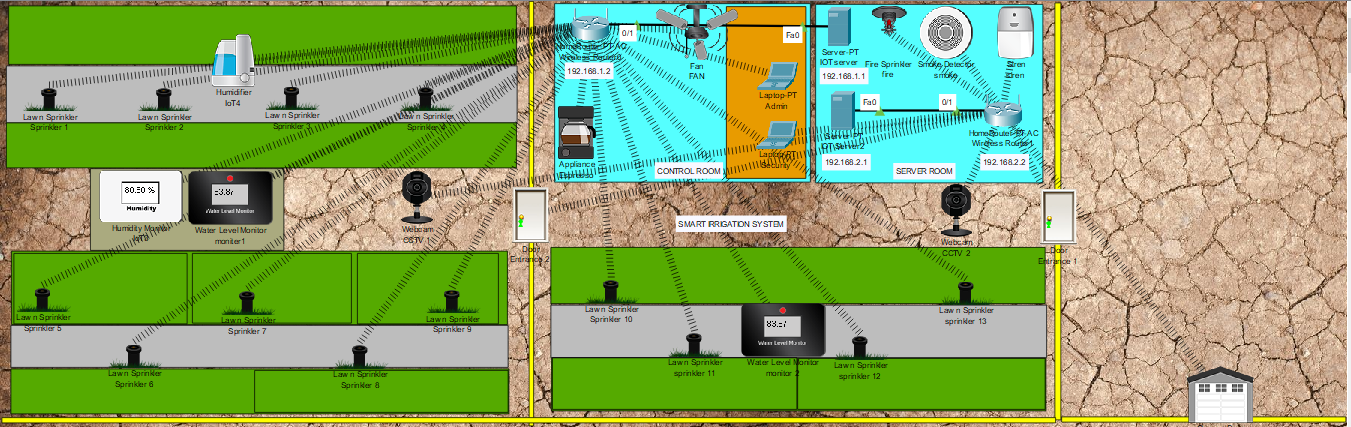
\includegraphics[width=15cm]{Design.png}
\caption{Design of Smart irrigation system}
\end{figure}
\subsection{Tools And Technologies}
With regards to the implementation of IoT devices, the used communication technologies could be considered as a vital and imperative point to attain successful operations. These are the tools and technology which was used to make this project: \cite{jakaria}
\begin{itemize}
    \item Cisco Packet Tracer Software: This is a network simulation tool that allows you to design and simulate a network, including the smart irrigation system.
    \item Network devices: We will need a variety of network devices to create the smart irrigation system, including routers, switches, and wireless access points.
    \item Sensors and controllers: We will need sensors to measure the moisture content of the soil and weather conditions, as well as controllers to process the data and make decisions about when to open and close the valves.
    \item Communication: We will need to use wireless technology, such as Wi-Fi, and controllable devices to allow the different components of the system to communicate with each other and to allow for remote monitoring and control.
\end{itemize}
\subsection{IOT and Other Devices}
Internet of Things (IoT) devices can be used in a smart irrigation system to collect and transmit data from sensors, control the sprinklers and other components of the system, and allow for remote monitoring and control. Some examples of IoT devices that we used in the smart irrigation system include:
\begin{itemize}
    \item Water Level monitors, Humidity monitor
    \item Lawn Sprinklers, Humidifier
    \item IoT servers
    \item Home Routers
    \item End devices(Laptop)
    \item Fire sprinkler
    \item smoke detector
    \item siren
    \item Fan
    \item appliance
    \item Doors
    \item Webcam(cctv)
\end{itemize}
\section{Work Procedure}
\subsection{IOT Server and Devices Configuration}
To set up an IoT server, we need to follow these steps: \\
\begin{itemize}
    \item Drag and drop the necessary devices onto the workspace. This will typically include at least one IoT device and a server.
    \item Configure the server by assigning it an IP address and connecting it to the internet.
    \item Configure the IoT device by assigning it an IP address and setting up any necessary protocols for communication with the server.
    \item Connect the IoT device to the server using a router or switch.
    \item Need to make a registration server using the iot service
    \item Then need to Test the connection between the IoT device and the server to ensure that they are able to communicate with each other.
    \item to configure the lawn sprinkler and water level monitor we need to configure the wireless and global setting of these devices.
\end{itemize}
\begin{figure}[h]
    \centering
    
    \begin{minipage}{0.45\textwidth}
    \centering
    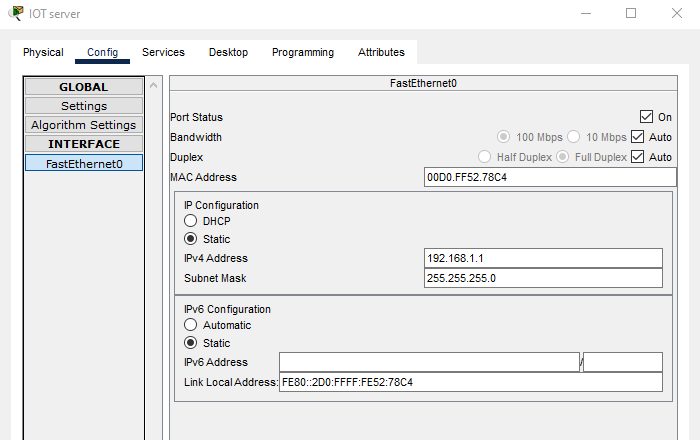
\includegraphics[width=1\textwidth]{1s.png}
    \caption{Configuration of IP addresses}
    \label{fig:1}
    \end{minipage}
    \hfill
    \begin{minipage}{0.45\textwidth}
    \centering
    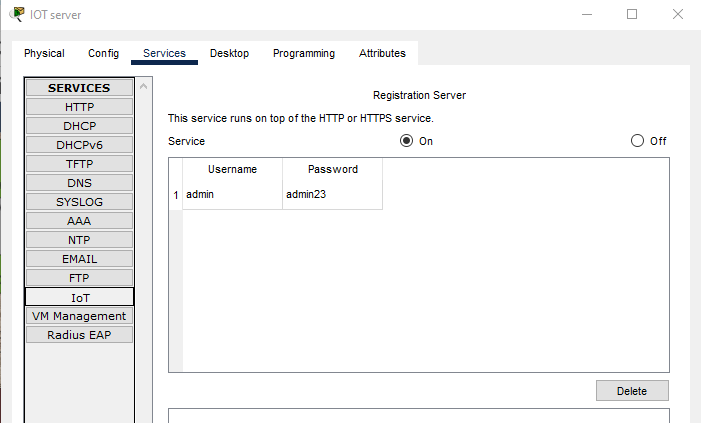
\includegraphics[width=1\textwidth]{2s.png}
    \caption{Configuration of IoT service}
    \label{fig:2}
    \end{minipage}  
\end{figure}
\newpage
\begin{figure}[h]
    \centering
    
    \begin{minipage}{0.45\textwidth}
    \centering
    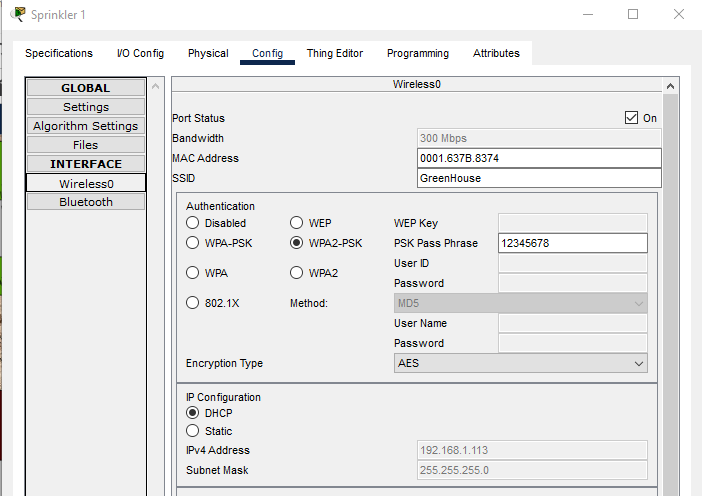
\includegraphics[width=1\textwidth]{iot/1d.png}
    \caption{Configuration of lawn sprinkler}
    \label{fig:3}
    \end{minipage}
    \hfill
    \begin{minipage}{0.45\textwidth}
    \centering
    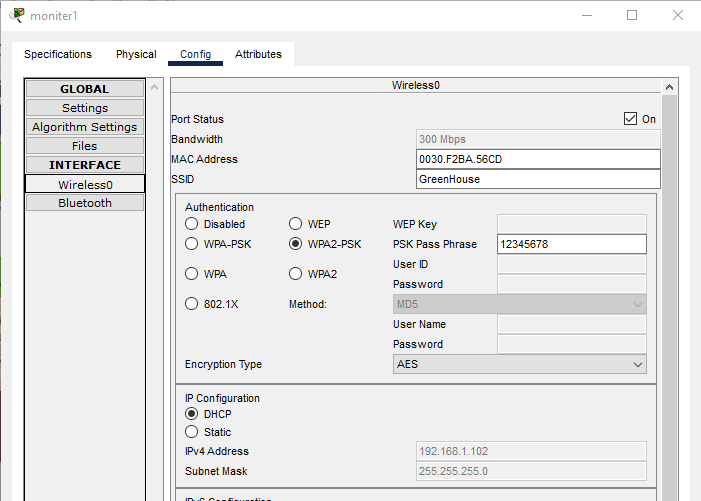
\includegraphics[width=0.8\textwidth]{iot/3d.png}
    \caption{Configuration of water level monitor}
    \label{fig:4}
    \end{minipage}  
    

\end{figure}

\subsection{Home Router Configuration}
To configure a wireless router, we need to follow these steps:\\
\begin{itemize}
    \item Drag and drop a wireless router onto the workspace.
    \item Connect the wireless router to the iot server using an Ethernet cable.
    \item Double-click on the wireless router to open its configuration window. In the configuration window, we need to go the GUI interface of the router.
    \item Need to Enable the wireless interface and set the desired wireless parameters, such as the SSID, channel, and security mode. Then need to go to the "Security" tab and configure the wireless security settings, such as the encryption type and password.
    \item Save the changes and close the configuration window.
    \item Then need to Connect a wireless client device to the wireless network to test the connection.
\end{itemize}
\begin{figure}[h]
    \centering
    
    \begin{minipage}{0.45\textwidth}
    \centering
    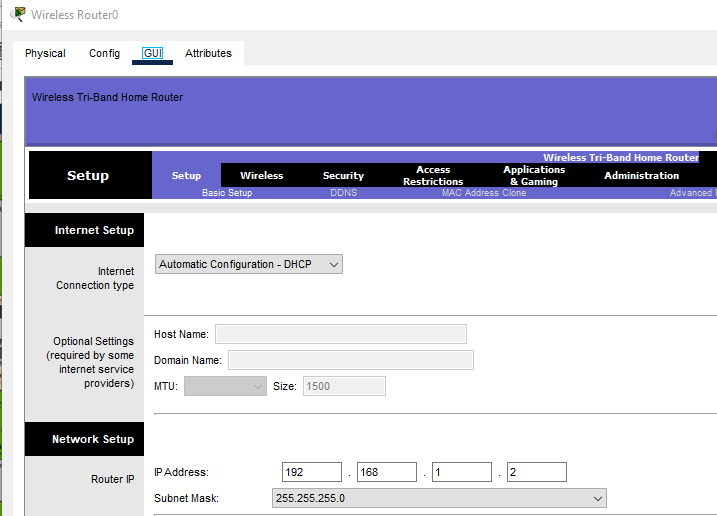
\includegraphics[width=1\textwidth]{Hr/1h.png}
    \caption{Configuration of IP address of router}
    \label{fig:5}
    \end{minipage}
    \hfill
    \begin{minipage}{0.45\textwidth}
    \centering
    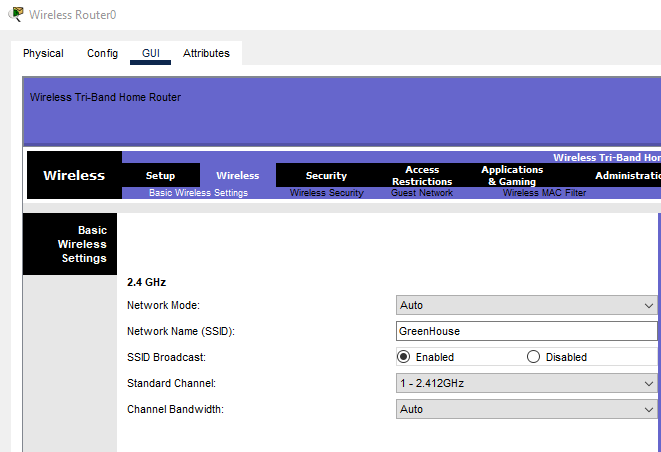
\includegraphics[width=1\textwidth]{Hr/2h.png}
    \caption{Configuration of wireless network}
    \label{fig:6}
    \end{minipage} 
      
\end{figure}
\newpage
\begin{figure}[h]
   
    \centering
    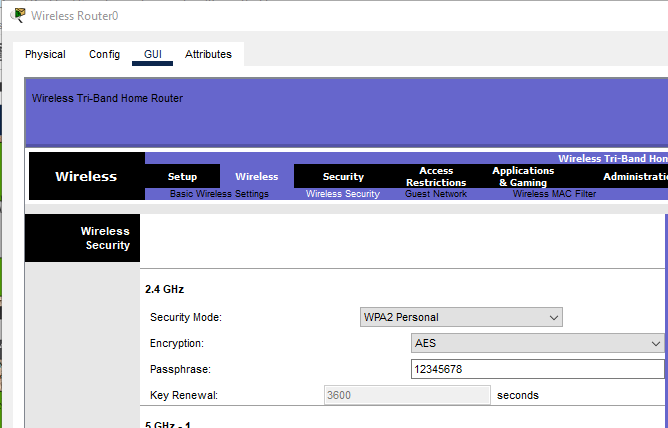
\includegraphics[width=0.50\textwidth]{Hr/3h.png}
    \caption{Configuration of wireless network security}
    \label{fig:7}
   
\end{figure}

\subsection{Admin and Security}
In this part the admin and security can control the overall system using an end device such as laptop.\\
\begin{itemize}
    \item to configure the end devices first need to connect the devices with a default gateway.
    \item then need to connect the devices with the wireless network created by the wireless home router.
    \item after connecting we need to go the web browser and go the desired registration server. For the admin part need to go to the iot server 1 and for the security part need to go to the second iot server.
    \item Admin can see all the connected devices. From there admin can set the conditions of the devices such as lawn sprinkler and water level monitor to work.
    \item for the lawn sprinklers to work need to set two conditon. One is for the lawn sprinkler to set On and other is to set Off. 
    \item lawn sprinklers will work by the condition of the water level monitor.
    \item For the security part there is a build in fire sprinkler in the server room. if there is a somke being detected then the siren will turn on and the fire sprinkler will start working.
    \item also for the security purpose the main entrance one will be unlocked. 
    \item the cctv cameras will work when it detects some movement over the doors.
\end{itemize}
\begin{figure}[h]
    \centering
    
    \begin{minipage}{0.45\textwidth}
    \centering
    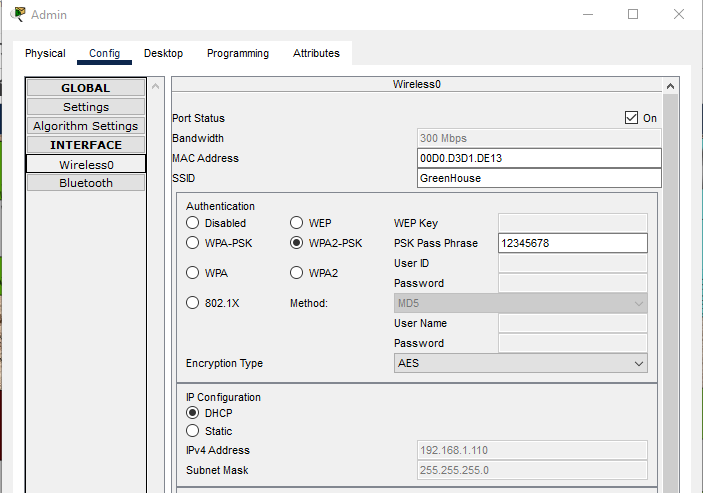
\includegraphics[width=1\textwidth]{As/1a.png}
    \caption{Configuration of end device}
    \label{fig:8}
    \end{minipage}
    \hfill
    \begin{minipage}{0.45\textwidth}
    \centering
    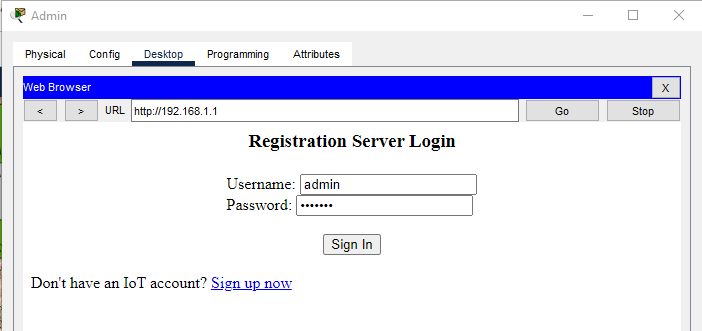
\includegraphics[width=1\textwidth]{As/2a.png}
    \caption{Accessing the server using laptop}
    \label{fig:9}
    \end{minipage} 

\end{figure}
\newpage
\begin{figure}[h]
    \centering
    
    \begin{minipage}{0.45\textwidth}
    \centering
    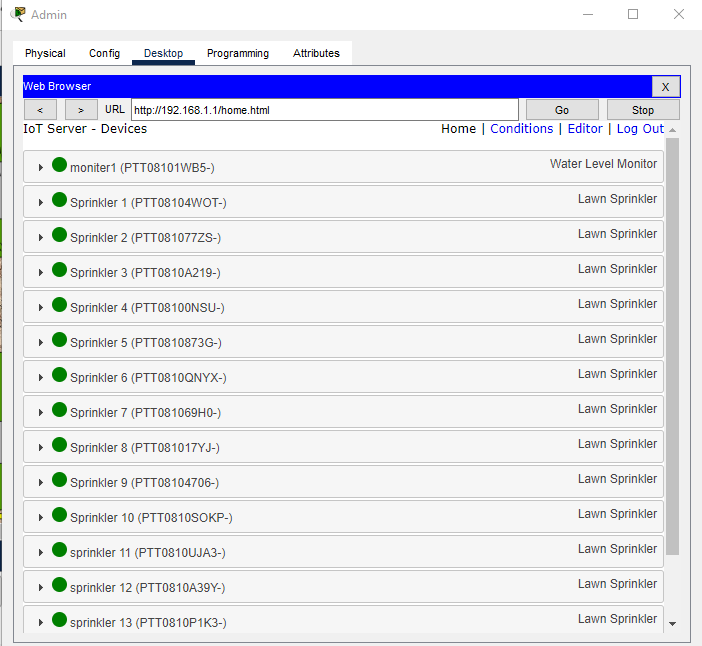
\includegraphics[width=1\textwidth]{As/3a.png}
    \caption{Connected devices in admin section}
    \label{fig:10}
    \end{minipage}
    \hfill
    \begin{minipage}{0.45\textwidth}
    \centering
    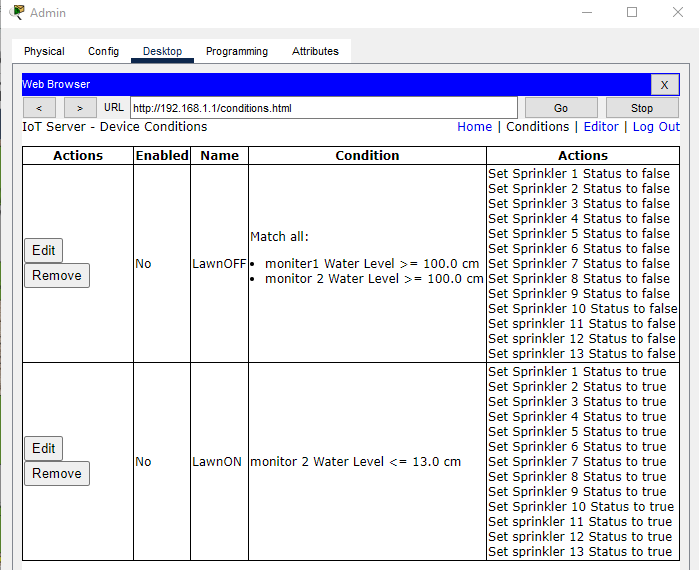
\includegraphics[width=1\textwidth]{As/4a.png}
    \caption{Configuration of Conditions}
    \label{fig:11}
    \end{minipage}

    \vspace{0.5cm}
    \begin{minipage}{0.45\textwidth}
    \centering
    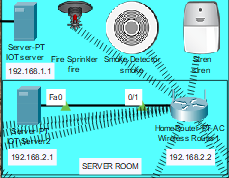
\includegraphics[width=1\textwidth]{As/1c.png}
    \caption{Security devices in the server room}
    \label{fig:12}
    \end{minipage}
    \hfill
    \begin{minipage}{0.45\textwidth}
    \centering
    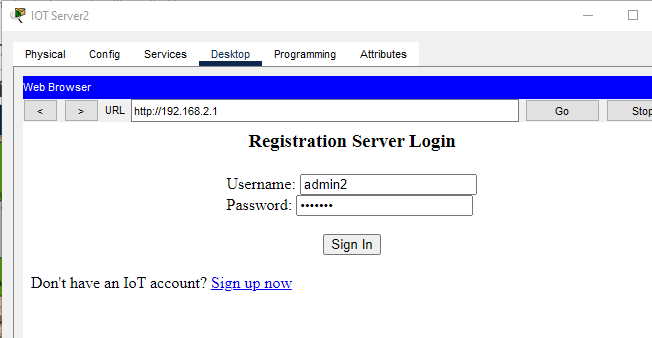
\includegraphics[width=1\textwidth]{As/2c.png}
    \caption{security section server}
    \label{fig:13}
    \end{minipage}

    \begin{minipage}{0.45\textwidth}
    \centering
    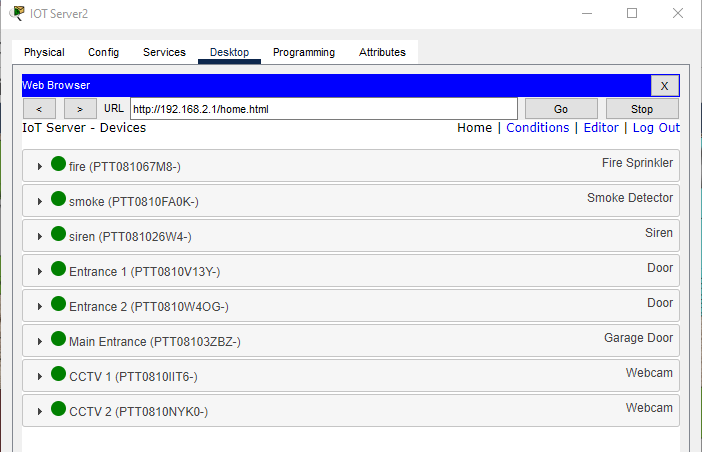
\includegraphics[width=1\textwidth]{As/3c.png}
    \caption{connected security devices}
    \label{fig:12}
    \end{minipage}
    \hfill
    \begin{minipage}{0.45\textwidth}
    \centering
    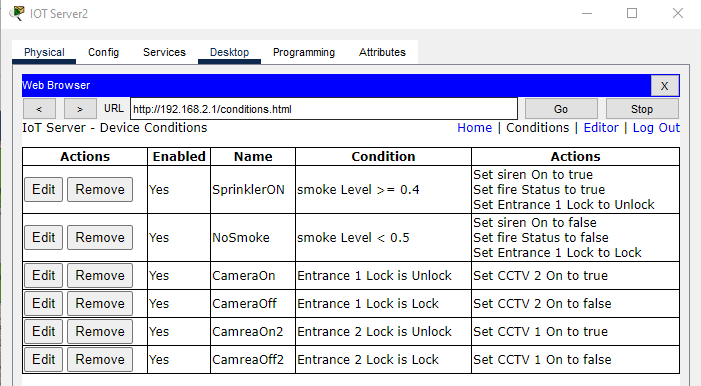
\includegraphics[width=1\textwidth]{As/4c.png}
    \caption{Configuration of Conditions for security devices}
    \label{fig:13}
    \end{minipage}
    
\end{figure}

\chapter{Performance Evaluation}
\section{Simulation Environment/ Simulation Procedure}
\begin{figure}[h]
    \centering
    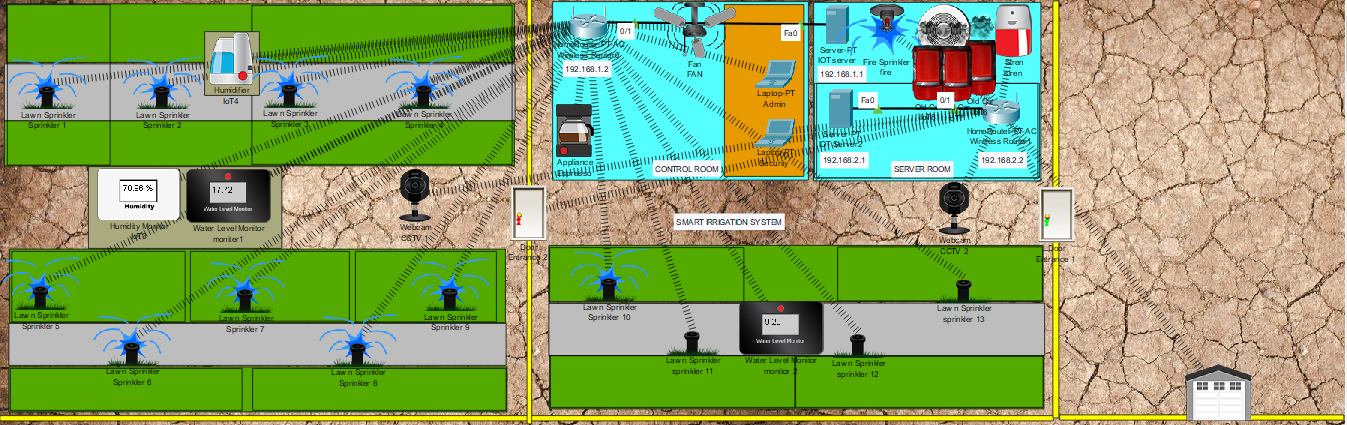
\includegraphics[width=1\textwidth]{Sim.png}
    \caption{Simulation of Smart Irrigation system}
    \label{fig:my_label}
\end{figure}
\section{Results and Discussions}
\subsection{Results}

\begin{figure}[h]

    \centering
   \begin{minipage}{0.40\textwidth}
    \centering
    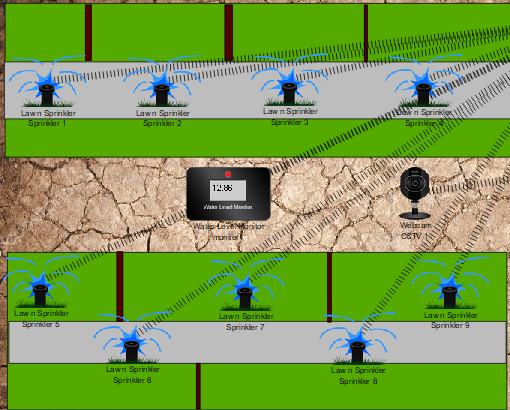
\includegraphics[width=1\textwidth]{rs/2.png}
    \caption{Output of Lawn sprinklers and monitor}
    \label{fig:my_label}
    \end{minipage}
    \hfill
    \begin{minipage}{0.40\textwidth}
    \centering
    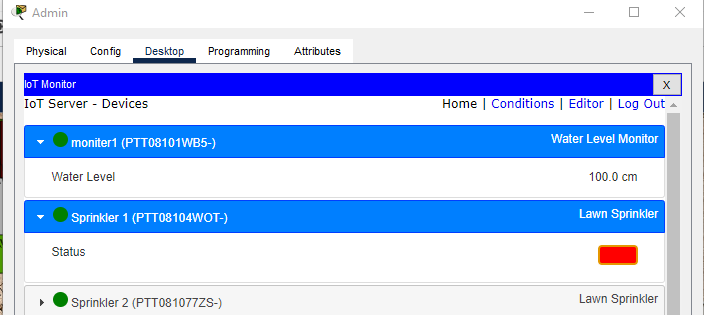
\includegraphics[width=1\textwidth]{rs/3.png}
    \caption{Conditions of Lawn sprinklers and monitors}
    \label{fig:my_label}
    \end{minipage}
\end{figure}
\newpage
\begin{figure}[h]
    \centering
   \begin{minipage}{0.40\textwidth}
    \centering
    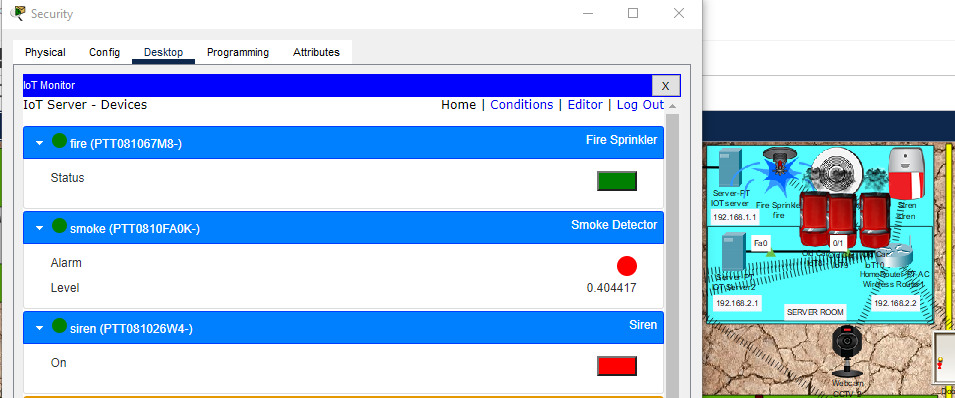
\includegraphics[width=1\textwidth]{rs/4.png}
    \caption{Security devices with conditions}
    \label{fig:my_label}
    \end{minipage}
    \hfill
    \begin{minipage}{0.40\textwidth}
    \centering
    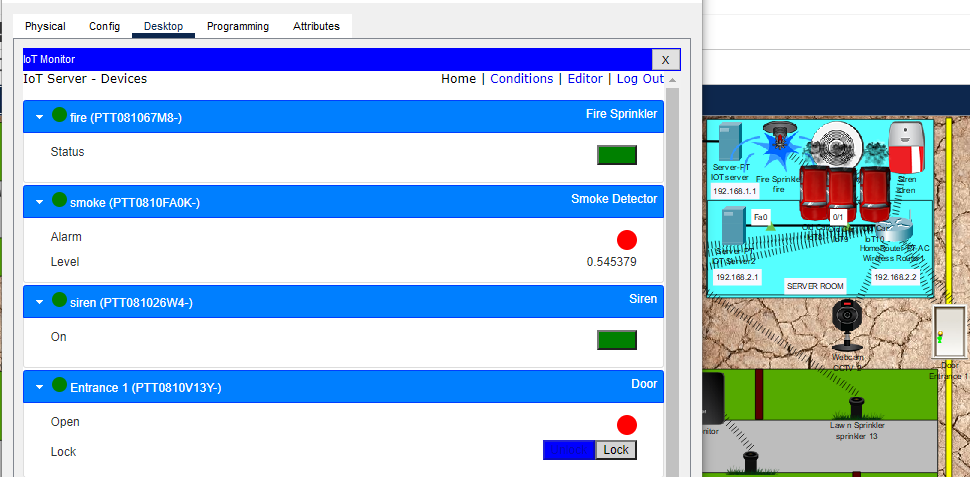
\includegraphics[width=1\textwidth]{rs/5.png}
    \caption{Security devices working}
    \label{fig:my_label}
    \end{minipage}
\end{figure}
\begin{figure}[h]

    \centering
   \begin{minipage}{0.40\textwidth}
    \centering
    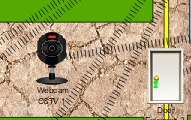
\includegraphics[width=1\textwidth]{rs/6.png}
    \caption{CCTV camera and entrance}
    \label{fig:my_label}
    \end{minipage}
    \hfill
    \begin{minipage}{0.40\textwidth}
    \centering
    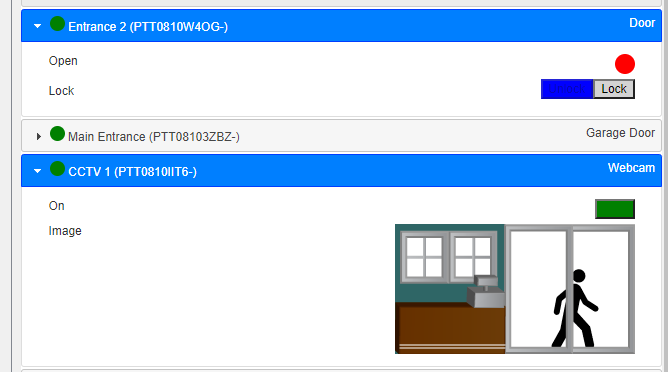
\includegraphics[width=1\textwidth]{rs/7.png}
    \caption{CCTV camera working with entrance door}
    \label{fig:my_label}
    \end{minipage}
\end{figure}
\vspace{0.5cm}
\subsection{Analysis and Outcome}
Smart irrigation systems use sensors, weather data, and other information to optimize watering schedules and reduce water waste in landscaping and agriculture. Smart irrigation systems can be programmed and controlled remotely, making it easy to adjust watering schedules and settings as needed. Overwatering or underwatering can lead to plant stress and reduced growth. Smart irrigation systems can help ensure that plants receive the right amount of water, leading to healthier plants. Overall, the use of smart irrigation systems can lead to significant water savings, improved plant health, and increased convenience.
\newpage
\chapter{Conclusion}
\section{Introduction}
The main purpose of smart irrigation system is to be an impactfull way of doing irrigation of crops. Surely it will reduce water waste. If we can implement this properly, then it will definitely be helpful to many people as well as many industries. The system can be monitored and adjusted remotely using a smartphone app or web portal, allowing users to make changes to the watering schedule as needed. So it can be remotely monitored, and for that reason, this system can be implemented wherever we want.
\section{Practical Implications}
There are several practical implications of using a smart irrigation system, including:\\
\begin{itemize}
    \item Smart irrigation systems can help reduce water usage by up to 50{\%} by adapting to local weather conditions and plant water needs. This can help save money on water bills and reduce strain on local water resources.
    \item By providing plants with the optimal amount of water, smart irrigation systems can help improve plant growth and reduce stress. This can lead to healthier plants and increased yields in agriculture.
    \item Smart irrigation systems can help reduce water waste and the associated environmental impacts, such as runoff and erosion.
    \item In addition to saving water, smart irrigation systems can also save money on energy costs by reducing the need for pumping and treating excess water.
\end{itemize}
Overall, the use of smart irrigation systems can have significant practical benefits for both individuals and communities.\\
\section{Scope of Future Work}
There are many areas where future work on smart irrigation systems could focus. Irrigation is a process of providing the desired amounts of water to agricultural land. This process is very beneficial in minimizing runoff or drought situations during the crop’s cultivation. Some possible areas of focus might include:\\ \cite{FutureSc95:online}
\begin{itemize}
    \item Smart irrigation systems rely on data analysis to optimize watering schedules, but there is still room for improvement in this area. For example, machine learning algorithms could be used to more accurately predict plant water needs based on a variety of factors.
    \item Smart irrigation systems could be integrated with other systems, such as weather forecasting systems, to provide more accurate and up-to-date data for optimizing watering schedules.
    \item Smart irrigation systems often rely on electricity to power sensors and control systems. Future work could focus on using renewable energy sources, such as solar or wind power, to power these systems.
    \item While smart irrigation systems are becoming more common, there is still room for increased adoption, particularly in areas with limited water resources. Future work could focus on promoting the use of smart irrigation systems and providing resources and support for those interested in implementing them.
    \item Smart irrigation systems have been developed and tested primarily in temperate climates, but there is a need for systems that are tailored to different climates and environments. Future work could focus on adapting smart irrigation systems to work effectively in a variety of different regions.
\end{itemize}
These are just a few examples of the many potential areas of focus for future work on smart irrigation systems. \\
\vspace{3cm}
\begin{center}
  \Large  {\bfseries Complex Engineering Problems (WP’s)}\\
  \end{center}
  \vspace{0.6 cm}
  \centering
  \begin{tabular}{|c|c|c|}\hline
      \textbf{No.} &\textbf{Name of the WP Attribute} & \textbf{Explain how you addressed this attribute}\\ \hline
       \textbf{WP1} & {Depth of knowledge required} & {Yes, it is required for this project} \\ \hline
       \textbf{WP2}& {Range of conflicting requirements} & {Balancing these conflicting requirements can be a major challenge}\\ \hline
       \textbf{WP3} & {Depth of analysis required} & {Yes, it is also required because it needed deep analysis} \\ \hline
       \textbf{WP4}& {Familiarity of issues} & {Yes, faced some issues regarding this project}\\ \hline
       \textbf{WP5} & {Extent of applicable codes} & { -----------------} \\ \hline
       \textbf{WP6}& {Extent of stakeholder involvement } & { ----------------- }\\ \hline
       \textbf{WP7} & {Interdependence} & {Yes,this project required some components that depends on another} \\ \hline
       
  \end{tabular}

\printbibliography

\end{document}
